\documentclass[master.tex]{subfiles}
 
\begin{document}

To treat the domain boundaries numerically ghost cells are implemented. Currently the simulation needs two ghost cells in every direction.

\subsection{X-Direction}
For the densities the following boundary conditions are employed:
\begin{equation}
    n_s(x) = \begin{cases}
        2 \cdot n_{s0}(0) - n_{s0}(-x) &\colon for \, x < 0 \\
        2 \cdot n_{s0}(x_L) - n_{s0}(2x_L-x) &\colon for \, x > x_L \\
    \end{cases}
\end{equation}
This enforces a mixed Dirichlet-Neumann boundary condition.
The parallel velocities are forced to equal zero at the boundaries.
For the potential a special boundary condition is employed:
\begin{align}
    \phi_e(x) = 0 \qquad &\colon for \, x = 0\\
    \partial_x\phi_e(x) = 0 \qquad &\colon for \, x = x_L \label{eq:boundary-potential-right}
\end{align}
The first condition fixes the absolute value of the potential and is necessary for the numerical solver to converge. This can be seen as a Coulomb gauge. This fixing may artificially create high gradients at the $x=0$ boundary and thus one needs to extend the boundary conditions of the densities into the domain. The second condition forces zero gradients in x-direction on the $x=x_L$ boundary. Since only the gradient of the potential appears as driving term in the equations those conditions for the potential move artificial dynamics to the left core region where they are easier to handle. 

\subsection{Y-Direction}
In Y-Direction (which is perpendicular to X and $\mathrm{B}$ but not exactly in poloidal direction) closed boundary conditions are implemented. One of the consequences is that there is an \textit{in and out flow} of vortices simulating turbulence incoming from the not simulated area of the poloidal slice. The length of Y-Direction needs to be chosen carefully such that vortices that are mirrored to the opposite do not interfere with themselves and that all important modes are possible (4x times x size) \cite{ScottFluxTube} \cite{ScottComputationMagneticallyConfinedPlasmas}.
\subsection{Z-Direction}
In Z-Direction there is a differentiation whether the X-coordinate lies in/on or outside the separatrix (last closed magnetic field line/flux surface).
\paragraph{In/On Separatrix}
Here we assume closed field lines and thus employ closed boundary conditions.
\paragraph{Outside of Separatrix}
To simulate \todo{Ref-Ribero-Scott} divertors outside the separatrix so called \textit{limiters} are simulated by not connecting the $z=0 \And z=n_z$ planes but rather using open boundary conditions for the densities and potential, and Dirichlet boundary conditions for the velocities. The situation is illustrated in \autoref{fig:boundary_conditions_z}
\begin{figure}[ht]
    \centering
    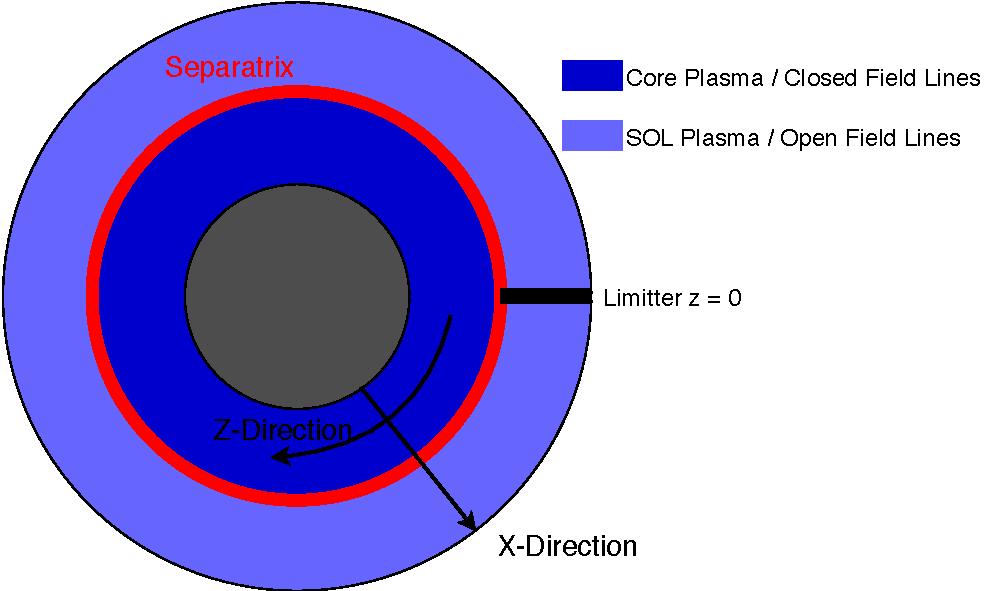
\includegraphics[width=\linewidth]{pdfs/boundary_conditions_z.pdf}
    \caption{Visualization of tokamak with separatrix and limiter}
    \label{fig:boundary_conditions_z}
\end{figure}

\end{document}